\documentclass[a4paper,12pt]{article}
\usepackage{graphicx}
\usepackage[margin=1.25in]{geometry}
\usepackage{listings}
\graphicspath{ {images/} }

\author{Ilyes Benarroum \\
Reda Nadir \\
Groupe 1
}
\title{FP-Growth}
\date{September 27}

\begin{document}
\maketitle
\section{Quel est FP-growth?}
FP-growth est une version améliorée de l'algorithme Apriori qui est largement utilisé pour d'exploration de données( génération des règles d'association). Il est utilisé comme processus analytique qui trouve des modèles ou des associations fréquents à partir d'ensembles de données(génération des règles d'association).
Il est utilisé comme processus analytique qui trouve des modèles ou des associations fréquents à partir d'ensembles de données.
Par exemple, Les données sur les transactions des épiceries peuvent avoir un schéma fréquent selon lequel les gens achètent généralement des chips et de l'eau ensemble.
L'algorithme Apriori produit des modèles fréquents en générant des ensembles d'éléments et en découvrant l'ensemble d'éléments le plus fréquent au-dessus d'un seuil de ''nombre minimal de support''.
Cela réduit considérablement la taille de l'ensemble d'éléments dans la base de données par un principe simple:

''Si un ensemble d'éléments est fréquent, tous ses sous-ensembles doivent également être fréquents.''

Cependant, l'algorithme Apriori présente un déficit majeur. L'utilisation d'Apriori nécessitait plusieurs analyses de la base de données pour vérifier le nombre de supports de chaque élément et ensembles d'éléments.
Lorsque la base de données est énorme, cela coûtera une quantité importante d'E / S disque et de puissance de calcul. Par conséquent, l'algorithme FP-Growth est créé pour combler ce déficit. Il scanne seulement la base de données deux fois et utilise une structure arborescente (FP-tree) pour stocker toutes les informations.
La racine représente null, chaque nœud représente un élément, tandis que l'association des nœuds est les jeux d'éléments avec l'ordre maintenu lors de la formation de l'arbre. L'arbre FP est concis et est utilisé pour générer directement de grands ensembles d'éléments. Une fois qu'un FP-tree a été construit, il utilise une approche récursive de division et de conquête pour extraire les ensembles d'éléments fréquents.

\section{Pseudocode et explication de l'arbre FP}
\begin{itemize}
    \item Étape 1: Déduisez les articles fréquents commandés. Pour les éléments de même fréquence, l'ordre est donné par ordre alphabétique.
    \item Étape 2: Construisez l'arbre FP à partir des données ci-dessus l'ordre est donné par ordre alphabétique.
    \item Étape 3: À partir de l'arbre FP ci-dessus, construisez l'arbre conditionnel FP pour chaque élément (ou ensemble d'éléments).
    \item Étape 4: Déterminez les modèles fréquents.
\end{itemize}

Voici un exemple qui illustre la création d’un arbre FP. Trouvez tous les ensembles d'éléments
fréquents avec un support  $\geq$2. Tout d'abord, recherchez tous les éléments avec un nombre de support $\geq$2.\\
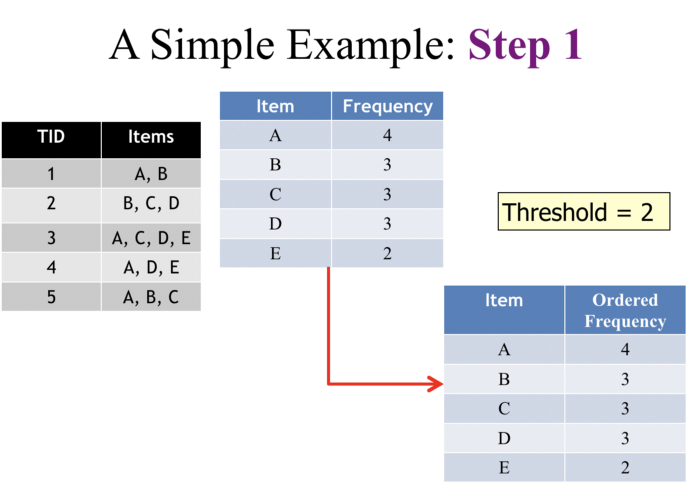
\includegraphics[width=\textwidth]{one}
Avant de construire l'arbre FP, réorganisez la transaction en fonction de la fréquence de leurs éléments. Lorsque vous commencez à construire l'arbre FP, nous devons créer une table d'en-tête qui enregistre l'emplacement de tous les nœuds d'élément avec une liste de liens. Chaque fois qu'un nouveau nœud est ajouté à l'arborescence, il doit être lié au dernier nœud avec le même élément. La table d'en-tête est essentielle pour créer une arborescence FP conditionnelle dans les étapes ultérieures.\\
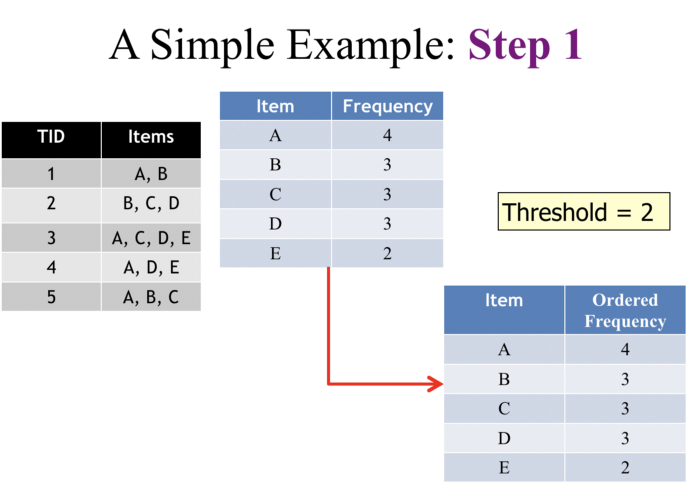
\includegraphics[width=\textwidth]{one}
Maintenant, nous avons scanné la base de données deux fois et construit l'arbre FP. Toutes les informations de transaction sont contenues dans l'arborescence. La seule chose qui reste à faire est de construire récursivement l'arbre FP conditionnel pour trouver tous les éléments fréquents avec un nombre de support supérieur à 2. Utilisez le tableau d'en-tête que nous avons créé à la dernière étape et commencez à partir de l'élément avec le nombre le moins la plupart (E, D, C, B, A).
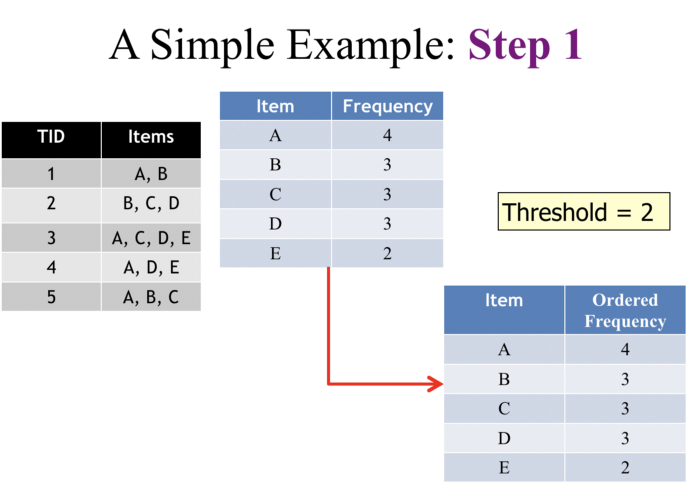
\includegraphics[width=\textwidth]{one}
Enfin, nous pouvons facilement générer tous les itemsets fréquents à partir de ces FP-arbres conditionnels {E}, {A, D, E}, {A, E}, {D, E}, {D}, {A, D}, { C, D}, {C}, {A, C}, {B}, {A, B}, {A}.
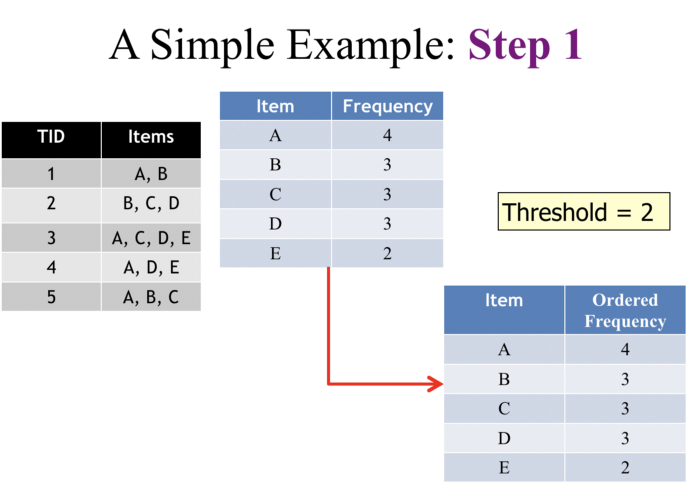
\includegraphics[width=\textwidth]{one}
\section{Implémentation Python}
Voici un exemple de code pour créer un FP-tree à partir de zéro et trouver tous les jeux d'éléments de fréquence dans Python 3.

En conclusion, FP-tree reste la méthode la plus efficace et la plus évolutive pour extraire l'ensemble complet des modèles fréquents dans un ensemble de données. La plupart des langages de programmation, y compris Python, R et même Pyspark, ont des bibliothèques bien prises en charge pour générer FP-tree.

\end{document}